\newpage
\section{Geschäftliche Grundlagen (10,75)}
\label{GeschäftlicheGrundlagen}
Das Marketing-Mix-Modell (\ac{MMM}) hat sich seit seiner Entstehung in den 1950er Jahren gewandelt. Mit der Verbreitung des digitalen Marketings hat sich das \ac{MMM} weiterentwickelt. Zuletzt wurde das \ac{MMM} durch die Fragmentierung der Media-Kanäle und den Signalverlust beeinflusst, die durch stetig wechselnde Datenschutz- und regulatorische Rahmenbedingungen verursacht wurden \cite[1]{MMMdef}. \par
In diesem Kapitel werden die geschäftlichen Grundlagen des \ac{MMM} vorgestellt. Der Nachfrageeffekt der Media-Kanäle wird mithilfe des \ac{MMM} berechnet, wofür fachliche Grundlagen und Kenntnisse über die aktuelle Situation erforderlich sind. Zuerst werden Fachbegriffe wie Marketing-Mix-Modell, Medium, Werbeausgaben und Markenimage definiert. Zudem wird das Purchase-Funnel-Modell vorgestellt, um ein besseres Verständnis für die Zielsetzungen der Media-Kanäle zu ermöglichen. Anschließend wird beschrieben, wie andere Unternehmen bei der Aufteilung der Mediaausgaben vorgehen. Zum Schluss wird die aktuelle Situation bei bonprix beschrieben und analysiert, um ein besseres Verständnis bei der Modellierung zu erhalten und die Anforderungen dabei besser zu verstehen.
\subsection{Einführung in das Marketing-Mix-Modell}
\label{EinführungInDasMMM}
Das Marketing-Mix-Modell (\ac{MMM}) basiert auf dem Konzept des Marketing-Mix. Der Marketing-Mix ist ein Konzept im Marketing und hilft Unternehmen, Ausgaben zu optimieren und die Kapitalrendite (\ac{ROI}) zu maximieren. Zudem erfasst er Marketingeffekte und identifiziert Investitionen, die langfristiges Wachstum fördern. Marketing-Manager steuern diese Variablen, um den Verkauf zu beeinflussen. \par
Der \textit{Mix} im Marketing-Mix verweist auf die Kombination der klassischen \textit{4Ps} im Marketing: Product, Price, Place and Promotion (dt. Produkt, Preis, Distribution und Kommunikation) \cite[S. 110]{akinkunmi2018data}. Produkt beschreibt, wodurch sich die Waren eines Unternehmens von Konkurrenzprodukten abheben, etwa durch Produkteigenschaften, Qualität, Design oder Wartung. Kommunikation umfasst unter anderem die Produktpräsentation mittels Werbung und Messen. Der Preis wird mit Hilfe von Strategien festgelegt, die von dem Produktlebenszyklus, den Eigenschaften des Produktes, dessen Nutzen und  konkurrierenden Produkten beeinflusst werden. Die Distribution beschreibt den Zustellungsbereich eines Produkts, der durch Faktoren wie Vertrieb, Verfügbarkeit und Erreichbarkeit bestimmt wird \cite[109--110]{akinkunmi2018data}. \par
Die Entwicklung des Marketing-Mix wurde geprägt durch die Suche nach der optimalen Allokation der Marketingausgaben. Dazu dienen Fragen wie: Was für eine Kombination von Marketing-Mix-Variablen verbessert die Kennzahlen wie Unternehmensumsatz oder Marktanteil am Gewinn? Wie reagieren diese auf die Ausgaben dieser Variablen? Auf Grundlage dieser Fragen haben Forscher ein Modell entwickelt, das diese Problematik behandelt. Das \ac{MMM} verwendet vergangene Daten, um valide Schlussfolgerungen zu ziehen und bessere Marketingstrategien für die Zukunft zu entwickeln. \par
In der heutigen Zeit wird das Bestimmen des effizientesten \ac{MMM} komplexer aufgrund der neuen Marketingstrategien und der Komplexität von computergestützten Daten. Das \ac{MMM} verwendet häufig multiple Regressionsmodelle, um die optimale Kombination der Marketing-Mix-Variablen vorherzusagen. Der Einsatz eines Regressionsmodells unterstützt dabei, den Einfluss unabhängiger Variablen wie Verkaufsförderung und Werbekosten auf die abhängige Variable, beispielsweise die Nachfrage, zu analysieren \cite[110]{akinkunmi2018data}. \par
Ein entwickeltes Regressionsmodell beschreibt die Beziehung zwischen den Variablen und kann eingesetzt werden, um eine Verkaufsprognose zu erstellen. Das Modell kann auch identifizieren, welche Koeffizienten der unabhängigen Variablen einen starken Einfluss auf den Kaufwunsch der Kunden haben. Dabei können unterschiedliche Eingabe-Variablen für das \ac{MMM} verwendet werden. Dazu gehören neben wirtschaftlichen Daten wie der Zins- oder Inflationsrate auch industrielle
Daten wie Preis, Konkurrenz und Services. Marktdaten wie Verkauf, Umsatz, Gewinn,\ac{ROI} sowie die Zielgruppendaten sind mögliche Variablen. Die Stabilität des Modells wird durch die Genauigkeit der Daten gegeben. 
\subsection{Werbewirkungen im Marketing-Mix-Modell}
\label{WerbeeffekteImMMM}
Verschiedene Werbewirkungen können in der Analyse vom \ac{MMM} entdeckt werden. In \cite{Pandey2021MMM} werden verschiedene Werbewirkungen im \ac{MMM} vorgestellt. Der aktuelle Effekt bezeichnet die unmittelbare Werbewirkung einer Maßnahme auf die Verkaufszahlen. Ähnlich einem Werbepuls führt er zu einer kurzfristigen Veränderung der Verkaufszahlen. Nach \cite{Pandey2021MMM} belegen Forschungsarbeiten, dass dieser Effekt im Vergleich zu anderen Marketingfaktoren klein und fragil ist. So ist die Wirkung von Preisänderungen beispielsweise 20-mal stärker als die von Werbung. Dadurch wird der Einfluss von Werbung oder Medien leicht durch Rauschsignale in den Daten überdeckt. Eine zentrale Herausforderung für Forscher besteht daher darin, Modelle sorgfältig zu gestalten, um Verzerrungen zu vermeiden und auch schwache Effekte zu berücksichtigen \cite[785]{Pandey2021MMM}. \par
Neben dem aktuellen Effekt gibt es auch einen Carryover-Effekt. Dieser Effekt bezieht sich auf den Teil der Wirkung, der in den Zeiträumen nach der Werbeexposition auftritt. Die Auswirkungen einer Werbemaßnahme sind nicht sofort in höheren Verkaufszahlen erkennbar, sie summieren sich über längere Zeiträume hinweg. Er kann durch verschiedene Faktoren verursacht werden, wie beispielsweise verzögerte Konsumreaktion, verzögerte Exposition oder durch Mund-Propaganda. Der Carryover-Effekt variiert in seiner Intensität. Das bedeutet, dass dieser Effekt manchmal genau so stark oder sogar stärker als der aktuelle Effekt der Werbung sein kann \cite[785]{Pandey2021MMM}.
\begin{figure}[H]
    \centering
    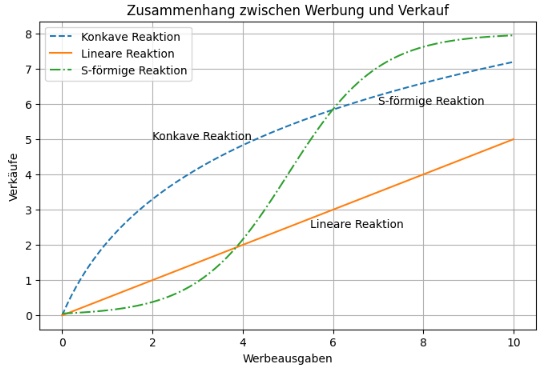
\includegraphics[width=0.75\linewidth]{images/formeffekt.png}
    \caption{Zusammenhang zwischen Werbung und Verkauf, angelehnt von \cite[1]{Pandey2021MMM}}
    \label{fig:formeffekt}
\end{figure}
\noindent
Der Form-Effekt bezieht sich auf die Veränderung der Nachfrage in Reaktion auf steigende Werbeintensität. Der Effekt kann verschiedene Formen annehmen: linear, konkav (mit abnehmendem Anstieg) und S-förmig (siehe \autoref{fig:formeffekt}). \cite{Pandey2021MMM} erläutert, dass die S-förmige Kurve als am wahrscheinlichsten angesehen wird. Dies weist darauf hin, dass eine Mindestschwelle in der Werbung erforderlich ist, um wahrgenommen zu werden, und dass eine erhöhte Werbeintensität ab einem bestimmten Punkt nicht notwendigerweise zu höheren Verkaufszahlen führt. Der Markt könnte gesättigt sein und Verbraucher könnten aufgrund von Überexposition ermüden \cite[786--787]{Pandey2021MMM}. \par
Ferner besteht auch der Wettbewerbseffekt. Dieser beschreibt, dass Werbung in freien Märkten stattfindet und wie die Zielmarke auf die Werbung konkurrierenden Marken reagiert. Unter fairen Marktbedingungen werden erfolgreiche Innovationen oder Werbekampagnen einer Marke schnell nachgeahmt. Die Wettbewerbswerbung erhöht Konkurrenzdruck, nimmt Marktanteile und verringert die Wirksamkeit der Werbung der Zielmarke. Eine isolierte Betrachtung der Zielmarke kann zu einer Fehlschätzung ihrer Effektivität führen aufgrund des wettbewerbsintensiven Umfelds. Neben dem Verdrängungseffekt der Wettbewerbswerbung kann die Werbewirkung der Zielmarke auch durch ihre Marktposition oder Bekanntheit beeinflusst werden. Beispielsweise profitieren größere Marken aufgrund ihrer Bekanntheit und Loyalität stärker von der gleichen Werbeintensität. Ein seltenes Phänomen ist der Kategorie-Halo-Effekt, bei dem die Werbung für eine gesamte Kategorie die Nachfrage aller darin enthaltenen Marken positiv beeinflusst. Dies tritt vor allem in neu entstehenden Marktsegmenten auf, in denen Verbraucher noch wenig Bewusstsein für die Marke oder die Kategorie insgesamt haben \cite[787]{Pandey2021MMM}.
\subsection{Media Definition}
\label{Media-KanäleDefinition}
Media wird definiert durch Kommunikationsträger. Insbesondere Massenmedien ermöglichen es dem Kommunikator, einen größeren Empfängerkreis zu erreichen. Der Empfängerkreis ist zeitlich und räumlich von sich und dem Kommunikator getrennt, wird aber durch die gemeinsame Zuwendung zum Medium erreicht. Klassische Massenmedien bedürfen typischerweise physischer Medien wie Zeitungen, Hörfunk und Zeitschriften. Durch die Digitalisierung entstehen auch digitale Kommunikationsträger wie soziale Medien und Blogs. Diese ermöglichen einen \anf{viele zu vielen}-Austausch, bei dem Individuen und Unternehmen im Netzwerk gleichberechtigt kommunizieren. Diese Medienmodelle sind für das Unternehmen von Interesse, da sie innerhalb kurzer Zeit ein großes Empfängerpublikum ansprechen. Sie treten beispielsweise in Form von Werbe- und \ac{PR}-Kampagnen auf \cite{Kleinjohann2024}. \ac{PR} steht für Öffentlichkeitsarbeit und bezeichnet die Kommunikation zwischen Organisationen oder Personen mit deren Umwelt. Dabei wird der Beziehungsaspekt zwischen den Beteiligten hervorgehoben \cite{Büsching2014}. \par
Media-Kanäle werden in zwei Hauptkanäle, traditionelle Werbung und digitale Werbung, unterteilt. Die traditionelle Werbung wird definiert durch die Above-the-Line-Medien, die die Werbebotschaften einem breiten Publikum übermitteln. Die Above-the-Line-Medien umfassen Massenmedien wie traditionelles Fernsehen, traditionelles Radio, gedruckte Zeitungen, Magazine und Out-of-Home-Werbeformate. Out-of-Home-Werbung umfasst alle Werbeformen in öffentlichen Bereichen, während digitale Out-of-Home-Werbung internetbasierte Werbeformen sind. Zur digitalen Werbung gehören Medien, die über das Internet ihre Werbebotschaften an Internet-Nutzer übermitteln. Darunter fallen digitale Out-of-Home-Werbungen, digitale Werbebanner, digitale Audiowerbung, digitale Kleinanzeigenwerbungen, Werbungen in digitalen Videos und Suchmaschinen sowie Influencer-Werbung \cite{statista_werbung}. 
\subsection{Werbeausgaben in Deutschland}
\label{werbeausgaben}
In diesem Kapitel werden die Werbeausgaben beschrieben, um einen Überblick über den Werbemarkt zu geben. Werbeausgaben sind Ausgaben eines Unternehmens, um auf einer Werbefläche ihre Produkte oder Dienstleistungen zu bewerben. Die Werbeausgaben für Deutschland in 2025 werden auf 25,93 Milliarden Euro geschätzt, was einer Steigerung von 2,93 \% im Vergleich zum Vorjahr entspricht \cite{statista_werbung}. Werbeausgaben der Media-Kanäle beziehen sich auf Ausgaben für Werbefläche in einem Medium. 
\begin{figure}[H]
    \centering
    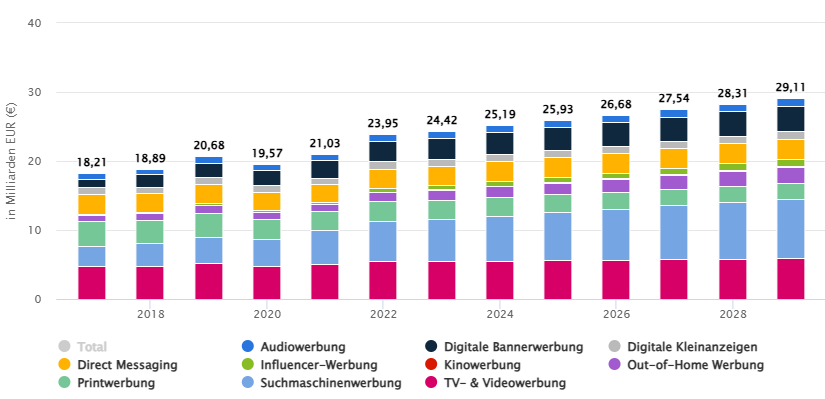
\includegraphics[width=0.90\linewidth]{images/werbede.png}
    \caption{Dokumentierte und geschätzte Werbeausgaben in Deutschland \cite{statista_werbung}}
    \label{fig:statistawerbungde}
\end{figure}
\noindent
Die \autoref{fig:statistawerbungde} zeigt die Verteilung der Werbeausgaben in Deutschland und veranschaulicht die verschiedenen Werbeformen. Das von Statista Insights erstellte Balkendiagramm visualisiert die Verteilung, Entwicklung und Prognose der Werbeausgaben in Deutschland. Im Jahr 2025 wird prognostiziert, dass die Suchmaschinenwerbung mit 6,92 Milliarden Euro an erster Stelle steht. Darauf folgt die TV- und Videowerbung mit 5,64 Milliarden Euro, gefolgt von der digitalen Bannerwerbung mit 3,26 Milliarden Euro. Die TV- und Videowerbung wird noch unterteilt in 1,53 Milliarden Euro in digitale Videowerbung und 4,12 Milliarden Euro in traditionelle TV-Werbung. Als Trend wird in Deutschland im Jahr 2029 63 \% der Werbeausgaben im digitalen Bereich erwartet und voraussichtlich 83 \% der Werbeausgaben entfallen auf Programmatic. Der Werbemarkt in Deutschland hat in den letzten Jahren ein starkes Wachstum verzeichnet. Laut einer Analyse von \cite{statista_werbung} haben verschiedene Faktoren wie Kundenpräferenzen, Markttrends, lokale Besonderheiten und makroökonomische Gegebenheiten maßgeblich zur Entwicklung dieses Marktes beigetragen. Insbesondere legen deutsche Verbraucher großen Wert auf Qualität und Authentizität, wobei personalisierte Werbung zunehmend an Bedeutung gewinnt. Gleichzeitig beeinflussen die zunehmende Digitalisierung und der Trend zu Influencer-Marketing das Werbeverhalten. Statista (2024) hebt hervor, dass auch der starke Fokus auf Datenschutz und die wachsende Bedeutung von Online-Werbung den Markt prägen \cite{statista_werbung}.
\subsection{Marke und ihre Auswirkung}
\label{markenimage} 
Die hohe Relevanz von Marken resultiert aus ihren vielfältigen Funktionen für Konsumenten. Aus ökonomischer Sicht verringern Marken die Such- und Informationskosten. Eine Marke kann für Kunden deshalb \anf{günstiger} sein. Aus Sicht des Kundenverhaltens dient die Marke zur Orientierung. Die Marke erhöht die Markttransparenz, dadurch identifizieren Kunden schneller und einfacher die für sie passenden Angebote \cite[2]{burmann2024}. \par
Ein zentrales Konzept in diesem Zusammenhang ist die Markenbekanntheit. Markenbekanntheit misst die Fähigkeit, sich an eine Marke zu erinnern. Ungestützte Markenbekanntheit (Brand Recall) ist das Erinnern an ein Markenzeichen wie Wortmarke, Bildmarke oder Wort-Bild-Marke. Gestützte Markenbekanntheit (Brand Recognition) ist das Erkennen der Marke nach einer akustischen und/oder visuellen Stützung. \cite[44]{burmann2024}. 

\subsection{Purchase-Funnel-Modell}
\label{PurchaseFunnelModell}
Das Purchase-Funnel-Modell beschreibt den trichterförmigen Verkaufsprozess. Das Purchase-Funnel-Modell ist eine Anlehnung an das AIDA-Modell. Das AIDA-Modell geht auf Lewis im Jahr 1899 zurück und beschreibt den Ablauf der Werbekommunikation in vier Stufen. Diese Stufen sind Aufmerksamkeit (Attention), Interesse (Interest), Verlangen (Desire) und Kauf (Action). Wie das AIDA-Modell bildet das \anf{Purchase Funnel}-Modell ebenfalls ein Stufenmodell von der Kontaktaufnahme bis zum Kaufabschluss. Das \anf{Purchase Funnel}-Modell wird generell in \anf{oberen Trichter}, \anf{mittleren Trichter} und \anf{unteren Trichter} aufgeteilt. Sie werden jeweils als \ac{ToFu}, \ac{MoFu} und \ac{BoFu} bezeichnet. Diese Phasen entsprechen den Zielen des AIDA-Werbewirkungsmodells: Aufmerksamkeitsgenerierung (Awareness), Interessensweckung (Interest) und Kauf (Action). Das Purchase-Funnel-Modell wird in \autoref{fig:purchase-funnel} visualisiert.
\begin{figure}[H]
    \centering
    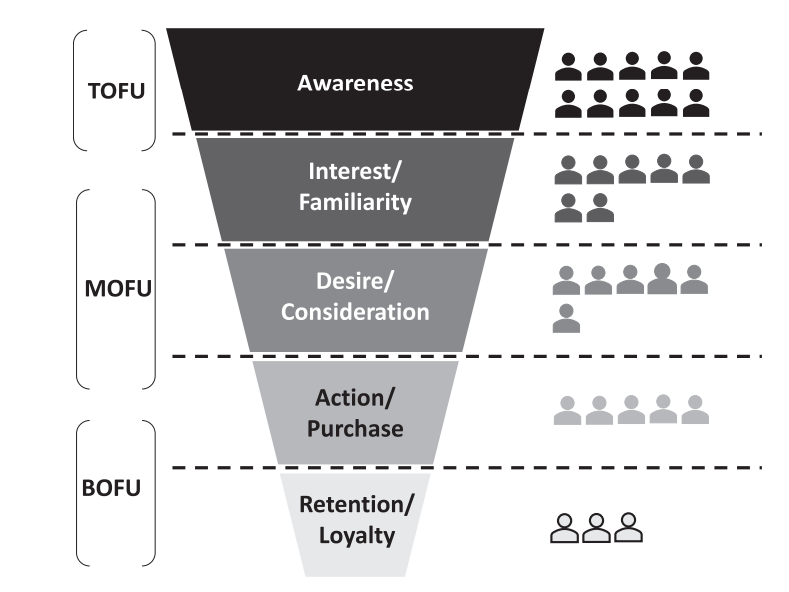
\includegraphics[width=0.75\linewidth]{images/Funnel.png}
    \caption{Purchase-Funnel-Modell \cite{Kleinjohann2024}}
    \label{fig:purchase-funnel}
\end{figure}
\noindent
Im oberen Teil des Trichters \ac{ToFu} wird der Konsument auf sein Problem oder Bedürfnis aufmerksam. Er sucht Lösungen in Form von Produkten und richtet sein Interesse auf das verfügbare Marktangebot. Im mittleren Teil des Trichters \ac{MoFu} bewertet der potenzielle Käufer das Angebot und nimmt Kontakt mit dem Anbieter auf oder nähert sich dem Verkaufsort. Im unteren Teil des Trichters \ac{BoFu} trifft der Konsument die Entscheidung, welches Produkt seine Bedürfnisse befriedigt und kauft es \cite{Kleinjohann2024}.
\subsection{Media-Kanäle in der Praxis}
\label{MediaKanäleInDerPraxis}
Mit wachsenden Kosten in Media-Kanälen gewinnt die Aufteilung der Kosten pro Kanal an Bedeutung. \par
Die Versicherung Generali hat in 2022 in ihrem \ac{MMM} herausgefunden, dass YouTube im Vergleich zu anderen Media-Kanälen überproportional stark auf die Steigerung von Markenbekanntheit, Markenpräferenz und Versicherungsabschlüssen einwirkt \cite{DasZusammenspielKundenloyalität2022}. Während des Covid-Lockdowns 2020 haben viele Menschen gelernt, YouTube für Erklärinhalte zu nutzen. Die YouTube-Videos der Versicherung hatten dabei einen positiven Einfluss auf alle gemessenen Loyalitätsmetriken. 44 \% der Nutzer, die diese Videos gesehen haben, wählten die Versicherung als ihre erste Wahl. Zudem erwogen 15 \% mehr Nutzer einen Anbieterwechsel, und 6 \% mehr waren bereit, eine Empfehlung auszusprechen \cite{DasZusammenspielKundenloyalität2022}. \par
Ein weiterer Bericht thematisiert den Wandel der Media-Kanäle. Eine von Nielsen im Auftrag von Google durchgeführte Metaanalyse zeigt, dass YouTube ein Effektivitätstreiber ist und das lineare TV beim \ac{ROI} übertrifft. Das Nutzungsverhalten für Media wird fragmentierter und das TV verliert an Bedeutung. Bei Personen unter 40 beträgt die Nutzung von linearem TV inzwischen weniger als 50 \% der gesamten Bewegtbildnutzung \cite{237097}.\par
Die Ergebnisse zur Abverkaufswirkung aus 144 \ac{MMM} wurden untersucht. Dabei zeigt sich, dass vier von fünf Unternehmen von höheren YouTube-Ausgaben in ihrem Marketing-Mix profitieren würden, um den Bewegtbild-ROI für TV und YouTube zu maximieren\cite{237097}. \par
Auch Offline-Medien haben eine Auswirkung auf das Kaufverhalten. Die zentrale Marktforschungsfirma von Deutschlands größter Mediaagenturgruppe, M-Science, entwickelte im Mai 2019 das Tool \anf{Crossoptimiser}. Das Tool behandelt das Problem der Wirkungsforschung, dass manche Einflussfaktoren auf das Werbeergebnis übersehen werden. Die gängigen Modelle ordnen messbare Erfolge allein Online-Kanälen zu. Beispielsweise werden die Bekanntheit, generierte Adressen und Kaufabschlüsse dem letzten Werbeklick der Nutzeraktivität im Netz zugeschrieben. Dieser Schluss übersieht die Wirkungsbeiträge, die Offline-Medien zu einem früheren Zeitpunkt im Wahrnehmungs- und Verkaufsprozess leisten. Vergleichbar mit dem Marketingtrichter (siehe \autoref{PurchaseFunnelModell}), finden und bestellen Nutzer online Produkte, weil sie zuvor eine Print- oder TV-Werbung gesehen haben. Karin Immenroth, die Geschäftsführerin und zugleich Marktforscherin der Group M, zieht ihre ersten Schlussfolgerungen nach einem Jahr Vorarbeit und hunderten durchgerechneten Kampagnen. Diese besagen, dass gerade bei Kunden mit einem hohen digitalen Werbeanteil der Wirkungsbeitrag von Offline oft stark unterschätzt wird. Je weiter sie im Marketingtrichter zurückforschen, desto stärker zeigt sich der Einfluss von Offline-Medien. Besonders bei Marken mit noch relativ niedrigen Awareness-Werten \cite[S. 4]{20190411492848}.
\par
Jollibee Food Corporation wurde 2020 die größte Fast-Food-Kette auf den Philippinen. Während einer Gesundheitskrise fiel der Verkauf im ersten Quartal um 10 \%. Um den Verkauf zu unterstützen, strebte das Unternehmen einen optimalen Media-Mix an. Es berichtete die gewertete Exposition der fünf üblichen Medien: TV, Magazin, lokale Zeitung, Plakat (\ac{ooh}) und soziale Medien. Jollibee gibt jährlich 9 bis 12 \% des Budgets für Werbung aus. Dabei werden die Kosten für lokale Zeitungen und Magazine kombiniert und auf unter 20 \% begrenzt. Zudem darf kein einzelner Kanal mehr als 30 \% des Budgets beanspruchen. Die Zielgruppen wurden in Haushalte mit niedrigem, mittlerem und hohem Einkommen unterteilt, mit Mindestwerten für erreichte Personen pro Peso je Medium. Mithilfe von Constraints wie maximalen Kosten wurde die optimale Kombination für eine maximale Gesamt-Reichweite mit einem Excel-Solver berechnet \cite{Tapiceria2020}. \par
Eine optimale Verteilung der Media-Kanäle kann dabei das maximale Potenzial jedes Kanals ausschöpfen. Unternehmen, die in wirtschaftlich herausfordernden Zeiten mit geprüfter und gesteigerter Effizienz der Maßnahmen in das Marketing investieren, sind überdurchschnittlich erfolgreich \cite{237097}. \par 
\subsection{Marketing-Mix-Modell bei bonprix} 
\label{Marketing-Mix-ModellBeiBonprix}
Bei bonprix modelliert das Marketing-Mix-Modell Daten ab 2020. \par
Vor der Entstehung des \ac{MMM} haben unterschiedliche Bereiche und Verantwortliche eigene Bewertungsansätze formuliert, um den jeweiligen Nachfrageeffekt zu bewerten. Beispiele für diese Bereiche sind Online-Marketing, Katalog und Media. Dabei wurde der Nachfrageeffekt der anderen Bereiche nicht berücksichtigt, und verschiedene Ansätze erschweren den direkten Vergleich der Kennzahlen. Später wurden die einzelnen Ländervertriebe organisatorisch zusammengeführt, um eine optimale Marketing-Budget-Strategie für ganz Europa zu erarbeiten. Es bestand das Bestreben, die Bewertungsansätze für den Nachfrageeffekt der Marketing-Bereiche zu vereinheitlichen. Hierbei soll das Marketing-Mix-Modell helfen. Das Marketing-Mix-Modell soll die Budgetentscheidungen unterstützen und zu einer besseren Verteilung des Budgets über die Länder hinweg beitragen.\par
\begin{figure}[H]
    \centering
    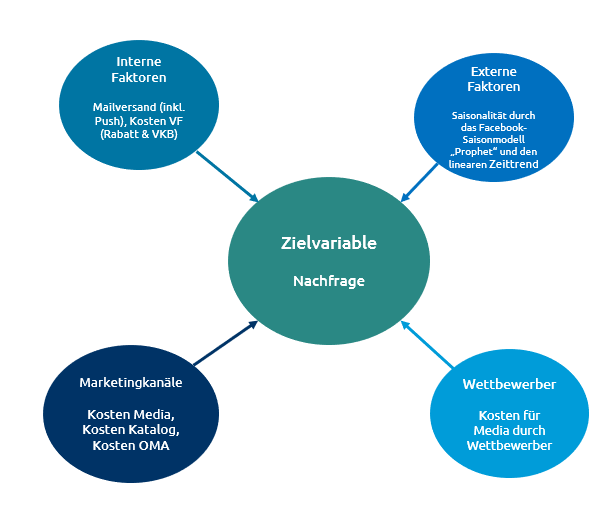
\includegraphics[width=0.85\linewidth]{mmm.png}
    \caption{Marketing-Mix-Modell bei bonprix, eigene Darstellung}
    \label{fig:mmmbonprix}
\end{figure}
\noindent
Das Marketing-Mix-Modell von bonprix berechnet den \ac{ROAS} für jeden Marketing-Kanal. Der \ac{ROAS} wird aus dem Quotienten der Nachfragesteigerung, die der Werbung zugeordnet werden und den Werbeausgaben errechnet \cite[2]{roas}:
\begin{equation}
ROAS = \frac{\text{Nachfragesteigerung, die der Werbung zugeordnet werden kann} \, (Euro)}{\text{Werbeausgaben} \, (Euro)}
\end{equation}
Jedes Jahr geben Marketer Milliarden von Euro für Online-Werbungen aus, um das Verhalten der Kunden zu beeinflussen. Die Online-Werbung hat einen Vorteil. Sie quantifiziert Kundenverhalten, das mit Online-Werbung verbunden ist. Das heißt, bezahlte Klicks, Website-Besuche und verschiedene Arten von Conversions können gesammelt werden. Diese Kennzahlen geben jedoch keinen Aufschluss darüber, wie sich die Kunden verhalten hätten, wenn keine Werbung geschaltet worden wäre. Um die Werbung zu verstehen, ist es wichtig, die Verhaltensänderung zu messen \cite[1]{roas}. Zu diesem Anlass wird der \ac{ROAS} als Kennzahl für den Werbewirkung eingesetzt. \par
Wie in \autoref{fig:mmmbonprix} beschrieben, werden unabhängige Variablen genutzt, um die Zielvariable \anf{Nachfrage} zu beeinflussen. Das Modell ähnelt dem in \autoref{EinführungInDasMMM} beschriebenen Modell. Die Variablen werden in vier Bereiche unterteilt: interne Faktoren, externe Faktoren, Marketingkanäle und Wettbewerber. Für die internen Faktoren verwendet das Modell Variablen wie Werbeaktionen und Mailversand. Das bedeutet, dass Verkaufsförderungen wie Rabatte, Versandkostenbefreiungen und die Anzahl an E-Mails, wie Newsletter und Trigger, genutzt werden. Für die externen Faktoren stehen die Saisonalität und der lineare Zeittrend zur Verfügung. bonprix entwickelte und verwendet einen Schätzwert, der die Saisonalität des Konsums vorhersagt. Für den linearen Zeittrend wird das Datum in fortlaufende Tage umgewandelt, wie Tag 1, Tag 2, ..., Tag n. Für die eigenen Marketingkanäle werden Ausgaben von anderen Kanälen berücksichtigt. Bonprix investiert in das \ac{OMA}, in Medienkanäle und in Kataloge. Da bonprix früher mit Katalogen geworben hat und es immer noch Leser gibt, investiert bonprix weiterhin in Kataloge. Das Online-Marketing ist ein führender Kanal. Täglich entstehen Kosten für das Online-Marketing, welches vergleichsweise einen großen Einfluss auf die Nachfrage hat. In 
\autoref{tab:mmmausgaben} ist zu erkennen, dass nach dem \ac{MMM} das Online-Marketing als steuerbarer Einflussfaktor den größten Einfluss auf die Nachfrage hat. Im ersten Zeitfenster, vom 1. Quartal 2020 bis zum 4. Quartal 2021, werden 36,5 \% der Nachfrage durch das Online-Marketing erklärt. Im Zeitraum vom 3. Quartal 2020 bis zum 2. Quartal 2022 sind es 29,8 \%, und im Zeitraum vom 1. Quartal 2021 bis zum 4. Quartal 2022 sind es 18 \%. Diese Werte werden abgeschwächt, da bonprix eine Sättigungsfunktion verwendet. Ab einer bestimmten Höhe der Ausgaben steigt die Nachfrageänderung langsamer, wodurch die ROAS für das Online-Marketing realistisch angepasst werden. Ferner besteht Media aus verschiedenen Unterkanälen, die in dem Kapitel \nameref{MediaKanäleBeiBonprix} ausführlicher beschrieben werden. Abschließend werden die Werbeausgaben von vier Konkurrenten im Bereich Online-Mode berücksichtigt.\par
Neben der Sättigungsfunktion werden auch andere Mechanismen eingesetzt, um die \ac{MMM}-Daten an die Realität anzupassen. Denn Werbeausgaben wirken nicht sofort und ihre Wirkung nimmt über die Zeit ab. Der Carryover-Effekt (siehe \autoref{WerbeeffekteImMMM}) oder Adstock wird mit einer Funktion integriert. Diese Funktion quantifiziert den verlängerten oder verzögerten Effekt von Werbung auf das Kaufverhalten der Verbraucher \cite{broadbent1979}. Adstock ist eine wichtige Komponente des \ac{MMM}. Auch der Abklingeffekt wird modelliert. Denn nach der Exposition einer Werbung wird das Bewusstsein für die Marke erhöht, jede neue Werbeeinblendung steigert das Bewusstsein auf ein neues Niveau. Der Abklingeffekt reduziert das Bewusstsein bis zum Basisniveau, es sei denn der Abklang wird verlangsamt oder gestoppt von erneuten Werbeeinblendungen \cite{Joseph2006Adstock}. Nach der Transformation wird ein Modell trainiert. Für das \ac{MMM} wird die robuste Huber-Regression verwendet, um den \ac{ROAS} zu berechnen. Die Huber-Regression wird im \autoref{huberregression} detaillierter erklärt. Während der Entwicklung von \ac{MMM} wurden auch andere Modelle erprobt. Allerdings waren die Ergebnisse nicht zufriedenstellend, daher wurde die Huber-Regression für die Berechnung des \ac{ROAS} aufgrund des nachvollziehbaren Konzepts sowie der besseren Ergebnisse beibehalten.
\begin{table}[H]
\centering
\renewcommand{\arraystretch}{1.3}
\setlength{\tabcolsep}{10pt}
\begin{tabular}{|l|c|c|c|}
\hline
\textbf{Einflussfaktor} & \textbf{Q1-20/Q4-21} & \textbf{Q3-20/Q2-22} & \textbf{Q1-21/Q4-22} \\ \hline
OMA                    & 36,5 \%               & 29,8 \%               & 18,0 \%               \\ \hline
Katalog                & 8,7 \%                & 8,4 \%                & 7,2 \%                \\ \hline
Media                  & 0,5 \%                & 1,5 \%                & 1,6 \%                \\ \hline
Mail                   & 2,5 \%                & 4,2 \%                & 3,0 \%                \\ \hline
Rabatt                 & 10,1 \%               & 13,1 \%               & 15,4 \%               \\ \hline
VKB                    & 6,6 \%                & 4,7 \%                & 4,7 \%                \\ \hline
Externe Faktoren       & 14,2 \%               & 19,7 \%               & 27,6 \%               \\ \hline
Konstante              & 21,0 \%               & 18,6 \%               & 22,5 \%               \\ \hline
\end{tabular}
\caption{\ac{MMM}-Ausgaben-Tabelle mit überlappenden Zeitfenstern von jeweils ungefähr zwei Jahren, eigene Darstellung}
\label{tab:mmmausgaben}
\end{table}
\subsection{Media-Kanäle bei bonprix} 
\label{MediaKanäleBeiBonprix}
Die Nachfrage, die den Media-Kanälen zugeordnet wurde, war zu Beginn der \ac{MMM}-Entwicklung sehr gering. Deshalb wurde die Effizienzanalyse ihrer Unterkanäle vernachlässigt. \par
Im \ac{MMM} von bonprix nehmen die Media-Kanäle nur einen kleinen Anteil der gesamten Nachfragen ein. Der Nachfrageanteil von Media wird im Folgenden mit etwa zweijährigen, überlappenden Zeitfenstern betrachtet: Zwischen dem ersten Quartal 2020 und dem vierten Quartal 2021 betrugen die Media-Nachfragen 0,5 \%. Sie stiegen im nächsten Zeitraum, vom dritten Quartal 2020 bis zum zweiten Quartal 2022, auf 1,5 \%. Zum Schluss erhöhten sich die Media-Nachfragen vom ersten Quartal 2021 bis zum vierten Quartal 2022 auf 1,6 \%. Um den Nachfrageeffekt der Media-Kanäle mit dem Nachfrageeffekt anderer Kanäle zu vergleichen, werden alle Nachfrageanteile in Form eines Balkendiagramms in \autoref{fig:mmmdiagramm} visualisiert. 
\begin{figure}[H]
    \centering
    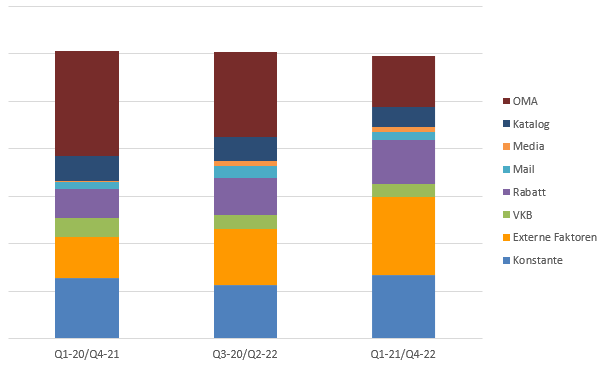
\includegraphics[width=0.75\linewidth]{images/mmmdiagramm.png}
    \caption{Nachfrageeffekt je Einflussfaktor aus dem \ac{MMM}-Modell, eigene Darstellung }
    \label{fig:mmmdiagramm}
\end{figure}
\noindent
Bei bonprix werden Mediaausgaben in Kampagnen umgesetzt. Das bedeutet, dass Media-Schaltungen aktiviert werden, wenn Kaufsaison ist und hohe Nachfrage besteht. Media-Schaltungen werden eingesetzt, um die maximale Reichweite beim Publikum zu erzielen. Die Dauer für die Aktivierung eines Media-Kanals ist ebenfalls begrenzt. Für das Online-Marketing fallen täglich Kosten an. Im Gegensatz zum Online-Marketing wird eine Media-Schaltung nur für einen begrenzten Zeitraum, etwa zwei Wochen oder einen Monat, aktiviert. In der Regel dauern Kampagnen vier Wochen. Radio wird für zwei Tage bis maximal zwei Wochen aktiviert. \par
Der Media-Mix wird anhand der Zielstellung der Kampagnen, \textit{Awareness} oder \textit{Consideration} (siehe \nameref{PurchaseFunnelModell}), abgeleitet. Ein Medium hat einen bestimmten Werbedruck und ein begrenztes Budget. Werbedruck wird definiert durch die Sichtbarkeit eines Unternehmens im Vergleich zu seinen Konkurrenten. Pro Jahr werden vier Kampagnen durchgeführt. In den vier Jahreszeiten finden jeweils eine Kampagne statt. Diese Kampagnen erfolgen jeweils zwischen März und April, Mai und Juni, September und Oktober sowie Oktober und November. Radio wird zum Beispiel zu bestimmten Aktionen wie Valentinstag oder Rabattaktionen aktiviert.\par
Die Anforderung für die Aufteilung der Mediaausgaben ist die Reichweite bei der Zielgruppe. Die Zielgruppe von bonprix sind 30-59-Jährige. Es wird angestrebt, mindestens 70\% der Zielgruppe pro Medium zu erreichen. Normalerweise wird diese Grenze überschritten. Außerdem wird der Werbedruck analysiert. Es wird beobachtet, wie viele Media-Schaltungen die Konkurrenten schalten, um weitere eigene Media-Schaltungen zu aktivieren. Dabei wird auf die eigene Sichtbarkeit eingegangen. Im \nameref{PurchaseFunnelModell} zielen Medienkampagnen darauf ab, zum \ac{ToFu} und \ac{MoFu} beizutragen. Das bedeutet, dass potenzielle Kunden auf die Marke aufmerksam werden und die Medienkampagnen ihr Interesse wecken sollen. \par
In der Media-Abteilung werden bereits \ac{KPI}s verwendet, um die Effektivität der verschiedenen Medienkanäle zu messen und zu bewerten. Dazu zählen gestützte und ungestützte Markenbekanntheit (\textit{Brand Awareness}), Markenberücksichtigung (\textit{Consideration}) und Werbeerinnerung (\textit{Ad Recall}). Die fachlichen Grundlagen werden in \nameref{markenimage} und \nameref{PurchaseFunnelModell} beschrieben. Im \ac{MMM} wird auch der \ac{ROAS} gerechnet. Allerdings wird das Medium als Ganzes betrachtet und nicht auf die einzelnen Kanäle wie TV, \ac{dooh}/\ac{ooh}, Radio usw. heruntergebrochen. Der \ac{ROAS} wird im Unternehmen für die übergeordnete Budgetplanung berücksichtigt, jedoch fehlen spezifische Daten, um ihn für die konkrete Mediaplanung einzusetzen. Um den \ac{ROAS} für die einzelnen Media-Kanäle zu berechnen, wird ein neues Modell entwickelt. Das Modell soll die Reichweite der Media-Schaltungen vorhersagen. Diese Entwicklung findet außerhalb, aber parallel zu dieser Arbeit statt. Dennoch ist es wichtig zu untersuchen, ob Media-Kanäle die Nachfrage positiv beeinflussen und somit Entscheidungen unterstützen können. Daraus ergibt sich die Forschungsfrage und der Kern dieser Arbeit, der in der Untersuchung des Nachfrageeffekts der Media-Kanäle besteht. Das Ergebnis dieser Arbeit soll zur Erweiterung des \ac{MMM} dienen. Die \ac{OLS}-Funktion und Huber-Regression sollen verwendet werden, um den \ac{ROAS} der Media-Kanäle im \ac{MMM} weiter zu berechnen. \par
In den Daten von \ac{MMM} sind auch die Kosten der jeweiligen Media-Kanäle enthalten. Jedoch werden Media-Schaltungen nicht nur aktiviert, wenn Kosten in den Daten anfallen. Anbieter wie ProSieben bieten beispielsweise auch kostenlose Werbespots an, wenn bestimmte Ausgaben erreicht werden. Das heißt, ungefähr 90\% der Media-Schaltungen werden mit Kosten dokumentiert und 10\% der Media-Schaltungen werden in den \ac{MMM}-Daten nicht mehr berücksichtigt. Die Nachfrageeffekte von diesen 10\% der Media-Schaltungen werden in dieser Arbeit nicht mehr analysiert. \par
Es existieren Herausforderungen bei dem Messen des Werbeeffekts für Media. Für TV wird ein Tool eingesetzt, das die Webshop-Besuche nach einer TV-Werbung zählt. Dabei wird die Erhöhung des Traffics im Webshop erkannt. Für Online-Werbungen ist es auch möglich, die Veränderung der Besucheranzahl zu dokumentieren. Jedoch ist es schwieriger, die Reichweite für \ac{dooh}, \ac{ooh} und Radio zu messen. Als \ac{KPI} für \ac{dooh}, \ac{ooh} und Radio wird die prognostizierte Reichweite herangezogen.